\section{Case Study}

% \begin{figure}
%     \centering
%     \includegraphics[width=0.96\textwidth]{figs/case.png}
%     \caption{Case study comparison between GPT-4o and MPPReasoner for CY-P450-2C9 substrate prediction. The figure demonstrates how RLPGR training enables systematic chemical reasoning with accurate predictions, while GPT4o suffer from several errors.}
%     \label{fig:case_study}
% \end{figure}

\begin{figure}
    \centering
    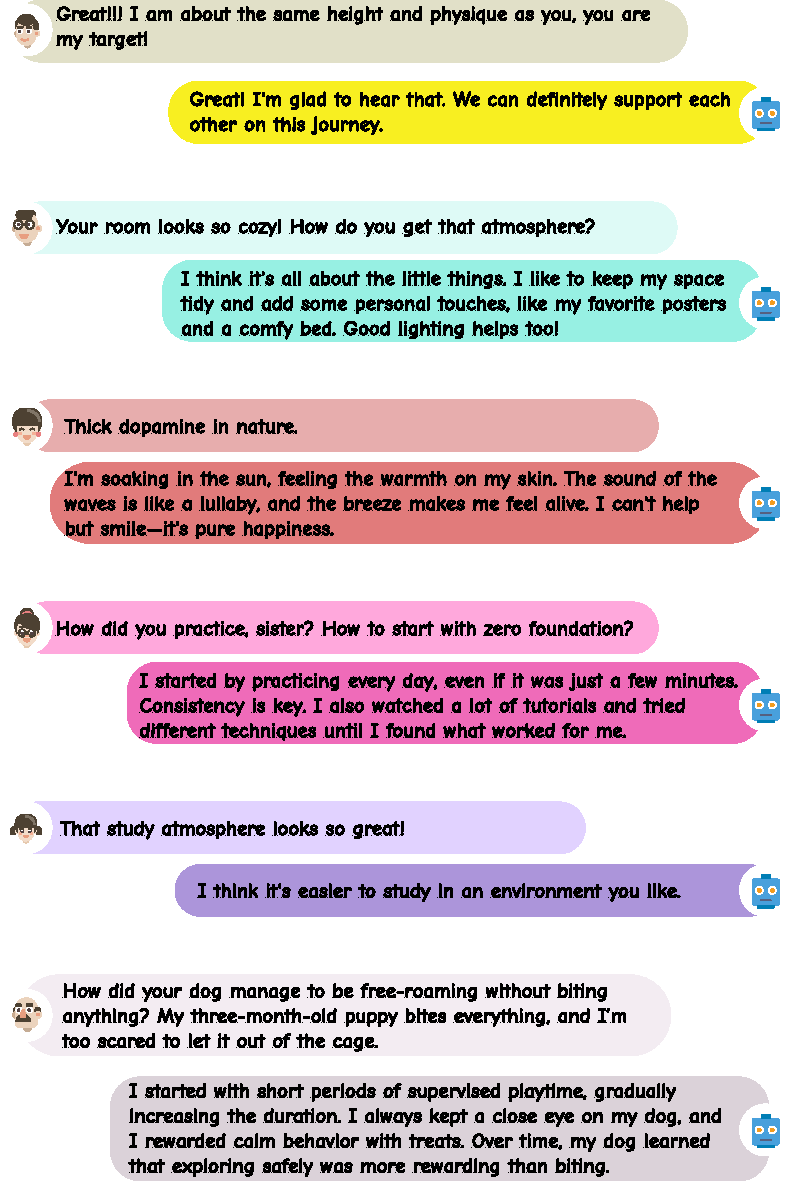
\includegraphics[width=0.98\textwidth]{figs/case1.png}
    \caption{Case study comparison between GPT-4o and MPPReasoner for CY-P450-2C9 substrate prediction. The figure demonstrates how RLPGR training enables systematic chemical reasoning with accurate predictions, while GPT4o suffer from several errors.}
    \label{fig:case_study}
\end{figure}


To illustrate the practical benefits of our chemical reasoning approach, Figure~\ref{fig:case_study} presents a representative case study comparing MPPReasoner with GPT-4o on CY-P450-2C9 substrate prediction. The comparison reveals fundamental differences in analytical quality: GPT-4o exhibits critical reasoning flaws including structural analysis errors (incorrectly assuming amide groups enhance binding affinity), overgeneralization (broadly claiming nitrogen-containing compounds show P450 compatibility), and incorrect reasoning patterns (unsupported statistical generalizations), ultimately leading to a wrong prediction. In contrast, MPPReasoner demonstrates systematic chemical reasoning through accurate molecular structure analysis (precise functional group identification), correct chemical principle application (referencing CYP2C9-specific LogP requirements and calculating steric hindrance), meaningful comparative analysis (connecting structural similarities to substrate labels), and logical consistency (integrating multiple evidence sources). This exemplifies how RLPGR's hierarchical rewards successfully cultivate domain-specific reasoning capabilities, enabling chemists to trust the model's mechanistic insights for practical applications.
